\iffalse
\let\negmedspace\undefined
\let\negthickspace\undefined
\documentclass[journal,12pt,twocolumn]{IEEEtran}
\usepackage{cite}
\usepackage{amsmath,amssymb,amsfonts,amsthm}
\usepackage{algorithmic}
\usepackage{graphicx}
\usepackage{textcomp}
\usepackage{xcolor}
\usepackage{txfonts}
\usepackage{listings}
\usepackage{enumitem}
\usepackage{mathtools}
\usepackage{gensymb}
\usepackage{comment}
\usepackage[breaklinks=true]{hyperref}
\usepackage{tkz-euclide} 
\usepackage{listings}
\usepackage{gvv}                                        
\def\inputGnumericTable{}                                 
\usepackage[latin1]{inputenc}                                
\usepackage{color}                                            
\usepackage{array}                                            
\usepackage{longtable}                                       
\usepackage{calc}                                             
\usepackage{multirow}                                         
\usepackage{hhline}                                           
\usepackage{ifthen}                                           
\usepackage{lscape}


\newtheorem{theorem}{Theorem}[section]
\newtheorem{problem}{Problem}
\newtheorem{proposition}{Proposition}[section]
\newtheorem{lemma}{Lemma}[section]
\newtheorem{corollary}[theorem]{Corollary}
\newtheorem{example}{Example}[section]
\newtheorem{definition}[problem]{Definition}
\newcommand{\BEQA}{\begin{eqnarray}}
\newcommand{\EEQA}{\end{eqnarray}}
\newcommand{\define}{\stackrel{\triangle}{=}}
\theoremstyle{remark}
\newtheorem{rem}{Remark}
\begin{document}
\parindent 0px
\bibliographystyle{IEEEtran}

\title{Assignment\\[1ex]11.9.1 - 9}
\author{EE23BTECH11220 - R.V.S.S Varun$^{}$% <-this % stops a space
}
\maketitle
\newpage
\bigskip

\renewcommand{\thefigure}{\theenumi}
\renewcommand{\thetable}{\theenumi}
\section*{Question}
Find $a_{9}$ in the sequence $a_{n}=\brak{-1}^{n-1}n^{3}$ 
\fi
 
\begin{table}[h]
    \centering
    \begin{tabular}{|c|c|c|}
    \hline
	 Symbol &Value&Description \\
        \hline
	 x\brak{0}&1&First term of the sequence\\
         \hline
	 x\brak{n}&$\brak{-1}^{n}\brak{n+1}^3u\brak{n}$& $\brak{n+1}^{th}$ term of the sequence \\
         \hline
         
    \end{tabular}

    
    \caption{Table of parameters}
    \label{tab:11.9.1.9.1}
\end{table}


To obtain $9^{th}$ term of the sequence put $n$=8 in x\brak{n}
\begin{align}
x\brak{8}=729
\end{align}
Using $Z$ transform,
\begin{align}
	X\brak{z}&=\sum_{n=-\infty}^{\infty}\brak{-1}^n\brak{n+1}^3u\brak{n}z^{-n}\\
	&=\sum_{n=-\infty}^{\infty}\brak{n+1}^3u\brak{n}\brak{-z}^{-n}\\
	&=\sum_{n=-\infty}^{\infty}\brak{n^3+3n^2+3n+1}u\brak{n}\brak{-z}^{-n}
\end{align}
Replace $z$ by $-z$ in \eqref{eq:uz},\eqref{eq:11.9.5.26.2},\eqref{eq:11.9.5.26.3},\eqref{eq:11.9.5.26.4}
\begin{align}
	u\brak{n}\xleftrightarrow{\mathcal{Z}}\frac{1}{1+z^{-1}},\abs{z}>1\\
	nu\brak{n}\xleftrightarrow{\mathcal{Z}}\frac{-z^{-1}}{\brak{1+z^{-1}}^2},\abs{z}>1\\
	n^2u\brak{n}\xleftrightarrow{\mathcal{Z}}\frac{z^{-1}\brak{z^{-1}-1}}{\brak{1+z^{-1}}^3},\abs{z}>1\\
	n^3u\brak{n}\xleftrightarrow{\mathcal{Z}}\frac{-z^{-1}\brak{1-4z^{-1}+z^{-2}}}{\brak{1+z^{-1}}^4},\abs{z}>1
\end{align}

\begin{align}
	X\brak{z}=\frac{z^{-2}-z^{-1}+1}{\brak{1+z^{-1}}^4},\abs{z}>1
\end{align}

\begin{figure}[h]
    \centering
    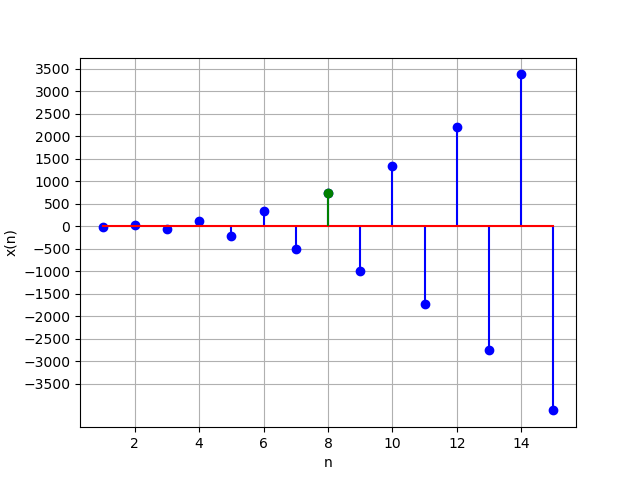
\includegraphics[width=1 \columnwidth]{ncert-maths/11/9/1/9/figs/graph.png} 
    \label{fig:11.9.1.9.1}
\end{figure}


